%% LyX 2.3.4.2 created this file.  For more info, see http://www.lyx.org/.
%% Do not edit unless you really know what you are doing.
\documentclass{article}
\usepackage[T1]{fontenc}
\usepackage[latin9]{inputenc}
\usepackage{geometry}
\geometry{verbose,tmargin=2cm,bmargin=2cm,lmargin=3cm,rmargin=3cm}
\usepackage{color}
\usepackage[spanish,english]{babel}
\addto\shorthandsspanish{\spanishdeactivate{~<>}}

\usepackage{url}
\usepackage{graphicx}
\usepackage[unicode=true,pdfusetitle,
 bookmarks=true,bookmarksnumbered=false,bookmarksopen=false,
 breaklinks=true,pdfborder={0 0 1},backref=false,colorlinks=false]
 {hyperref}

\makeatletter
%%%%%%%%%%%%%%%%%%%%%%%%%%%%%% User specified LaTeX commands.
\usepackage{charter}

\makeatother

\usepackage{listings}
\addto\captionsenglish{\renewcommand{\lstlistingname}{Listing}}
\addto\captionsspanish{\renewcommand{\lstlistingname}{Listado de c�digo}}
\renewcommand{\lstlistingname}{Listing}

\begin{document}
\title{Task 1: Motif Discovery using Prosite}
\author{\selectlanguage{spanish}%
Luis Garreta\\
Electiva de Bioinform�tica\\
MAESTR�A EN INFORM�TICA BIOM�DICA\\
Universidad del Bosque\\
Bogot�-Colombia}
\maketitle

\section{Goal}

The aims of this lab are to enable you to gain experience with sequence pattern discovery and pattern searching.

Databases and search tools:
\begin{itemize}
\item PROSITE is a database of protein families and domains. It consists of biologically significant sites, patterns and profiles that help to reliably identify to which known protein family (if any) a new sequence belongs. 
\item The ScanProsite tool allows users to scan protein sequence(s) (either from UniProt Knowledgebase (Swiss-Prot/TrEMBL) or PDB or provided by the user) for the occurrence of patterns, profiles and rules (motifs) stored in the PROSITE database, or to search protein database(s) for hits by specific motif(s)
\item PRATT at EBI, http://ca.expasy.org/tools/pratt/. A quick user guide is here. Note that pratt works by repeated pattern extension, generates regular expression patterns in a Prosite syntax, and can find several patterns which are descriptive of the input sequences. Moreover it can also refine (improve) the pattern set which it finds. 
\end{itemize}

\section{Problem}

A medical researcher has aligned a set of sequences that possibly contain an important protein motif (amino acids rather than DNA). The researcher needs the help of bioinformaticians to discover the unknown motif. The aligned sequences are:
\begin{center}
\begin{lstlisting}
RHSHYLPFRGGARNCIGTLLRFELLPDPTR
DPFSAYHFDGGARNCIGKQARLVVDTLREL
FDPGRARFFGGARNCIGQFAMKVLTLVRFE
DPSRFAPFDGGARNCIGFAMLKVGLRFELL
DSFADPRFSGGARNCIGQAMMIVLLRFELL
RAPSRSHFRGRARNRIGQFMEKASTLRELP
RFPSHHAFRGRARNPIGKQLTLLRFELLPD
PAPSRSHFPGRARNAIGKQFMEKAATLRDD
AGSSHSHFAGRARNFIGFAMNKVALTLRFE
\end{lstlisting}
\par\end{center}

If there is a significant motif, the researcher wants to confirm and know what protein motif it is and what its biological function is by using the PROSITE database, which is an annotated collection of motif descriptors dedicated to the identification of protein families and domains.

In this realistic exercise, we are going to:
\begin{itemize}
\item Construct a motif from aligned sequences
\item Buscar y confirmar el motivo en la base de datos de motivos de Prosite.
\item Use any hits that we find to make some other patterns characteristic of the retrieved set. These patterns will be regular expressions, generated using pratt.
\end{itemize}

\section{Protocol}
\begin{enumerate}
\item To discover the motif, you can modify the R script for discovering ADN motifs to work with protein motifs (aminoacids). Follow the next steps:
\begin{enumerate}
\item Create a string vector from the sequences

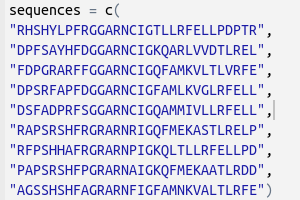
\includegraphics[scale=0.5]{img-stringVector}
\item Convert the string to a character matrix

\hspace{-2cm}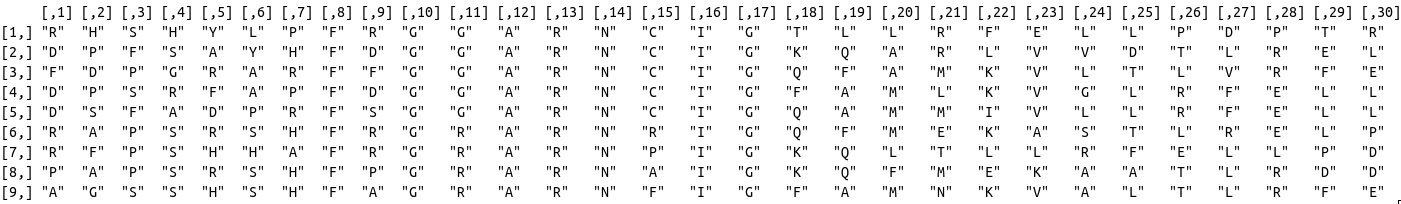
\includegraphics[scale=0.4]{img-char-matrix}
\item Calculate the position frequency matrix:
\begin{itemize}
\item Take into account that you are working with aminoacids instead of nucleotides.

{\scriptsize{}}
\begin{lstlisting}[basicstyle={\scriptsize},frame=lines]
aminos = c ("A","R","N","D","C","Q","E","G","H","I","L",
            "K","M","F","P","S","T", "W","Y","V","B","Z","X")
instead of
bases = c ("A","C","G","T")
\end{lstlisting}
{\scriptsize\par}
\item Add a low pseudocount to the frecuency matrix (0.01).

\begin{lstlisting}[basicstyle={\scriptsize},frame=lines]
freqMatrix = freqMatrix + 0.01
\end{lstlisting}

\end{itemize}
\hspace{-2cm}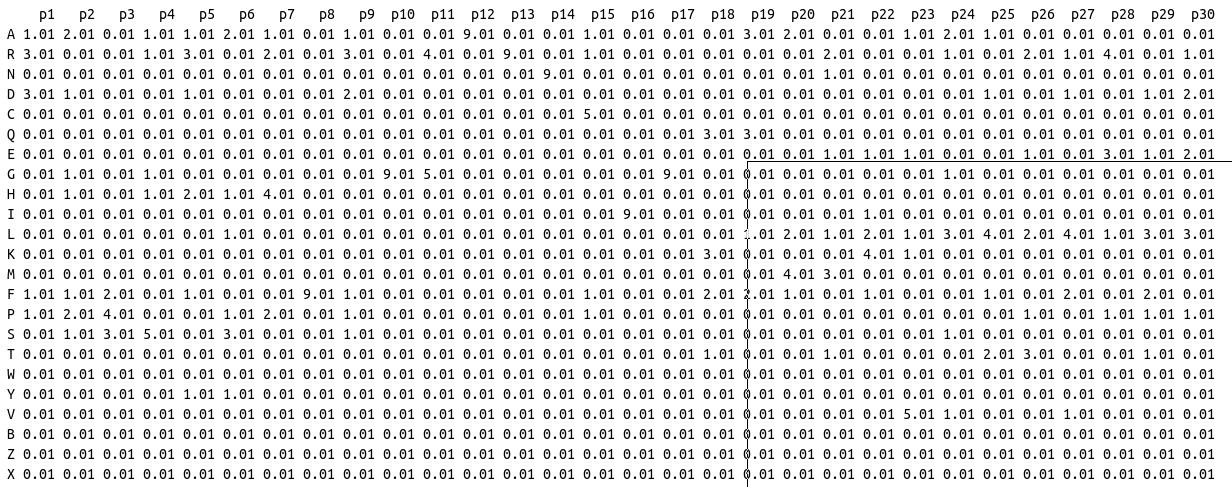
\includegraphics[scale=0.45]{img-freq-matrix}
\item Calculate de position weight matrix (PWM):
\begin{itemize}
\item Take into account the added pseudocount to normalize the frequencies:

\begin{lstlisting}[basicstyle={\scriptsize},frame=lines]
probMatrix = freqMatrix/(N+23*0.01)
\end{lstlisting}

\end{itemize}
\hspace{-2cm}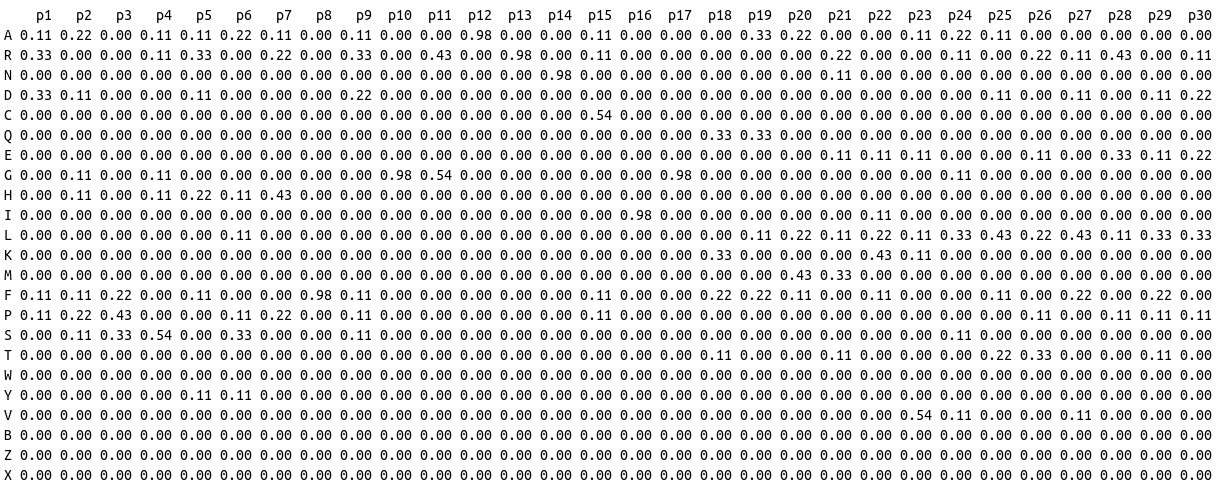
\includegraphics[scale=0.4]{img-prob-matrix}
\item Create the logo from the PWM, and from the logo construct the regular expression pattern. For the regular expresion take into account:
\begin{itemize}
\item The motif must start with a completely conserved aminoacid
\item The motif must end with a completely conserved aminoacid

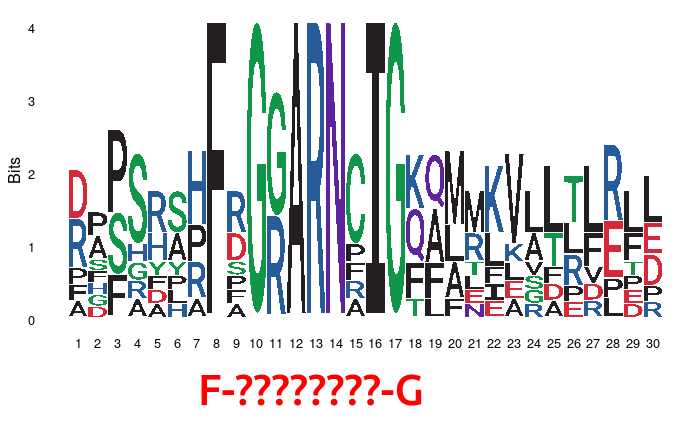
\includegraphics[scale=0.2]{img-logo}
\end{itemize}
\end{enumerate}
\item Now, search the motif in SwissProt using the ScanProsite (\url{https://prosite.expasy.org/scanprosite/}). Select \textbf{\emph{``Option 2''}} in the form and enter the motif to search sequences matches to this motif. 

\textcolor{blue}{Report the name of the motif and its biological function.}
\item Retrieve these hits in fasta format, go to ``STEP 3'' in the form, select maximum 10 sequences, and save them all in one file. To do this, You have to select either:
\begin{itemize}
\item ``FASTA'' output format, then select the sequences. 
\item ``Graphical view'' ``output format, then go to the page for each sequence, hit and click on the 'fasta' button, and save them all in one file. 
\end{itemize}
\textcolor{blue}{Report the sequences.}
\item Check that these sequences are specific to the search motif using the ScanProsite, select \textbf{\emph{``Option 1''}} in the form, paste the sequences into the ScanProsite input form to search for PROSITE collection of motifs in the sequences. 

\textcolor{blue}{Report the graphical view of the first result.}
\item Use PRATT (\url{http://www.ebi.ac.uk/pratt/}) as an automated method to construct regular expressions characterising these sequences. To get these regular expressions, using the last retrieved fasta sequences, copy them in the input form and submit to PRATT. Wait for results, and from them \textcolor{blue}{report the largest regular expresion}.
\item Finally. Search back into SwissProt with ScanProsite using the largest pattern and see what hits are obtained. 
\begin{itemize}
\item Do these searches return all of the original sequences?
\item What other sequences (if any) are identified by these patterns? 
\end{itemize}
\end{enumerate}

\end{document}
